%
% rueckprojektion.tex -- Rueckprojektion
%
% (c) 2021 Prof Dr Andreas Müller, OST Ostschweizer Fachhochschule
%
\documentclass[tikz]{standalone}
\usepackage{amsmath}
\usepackage{times}
\usepackage{txfonts}
\usepackage{pgfplots}
\usepackage{csvsimple}
\usepackage{mathrsfs}
\definecolor{darkgreen}{rgb}{0,0.8,0}
\usetikzlibrary{arrows,intersections,math}
\begin{document}
\def\skala{1}

\def\w{42.8}
\def\r{1.67}

\def\we{82.1}
\def\re{0.99}

\def\wc{-84.2}
\def\rc{1.62}

\def\wb{61.5}
\def\rb{1.56}

\def\d{0.1}
\begin{tikzpicture}[>=latex,thick,scale=\skala]
\clip (-7,-7) rectangle (7,7);

\begin{scope}[xshift=-3.7cm,yshift=3.7cm]
	\node at (0,0) {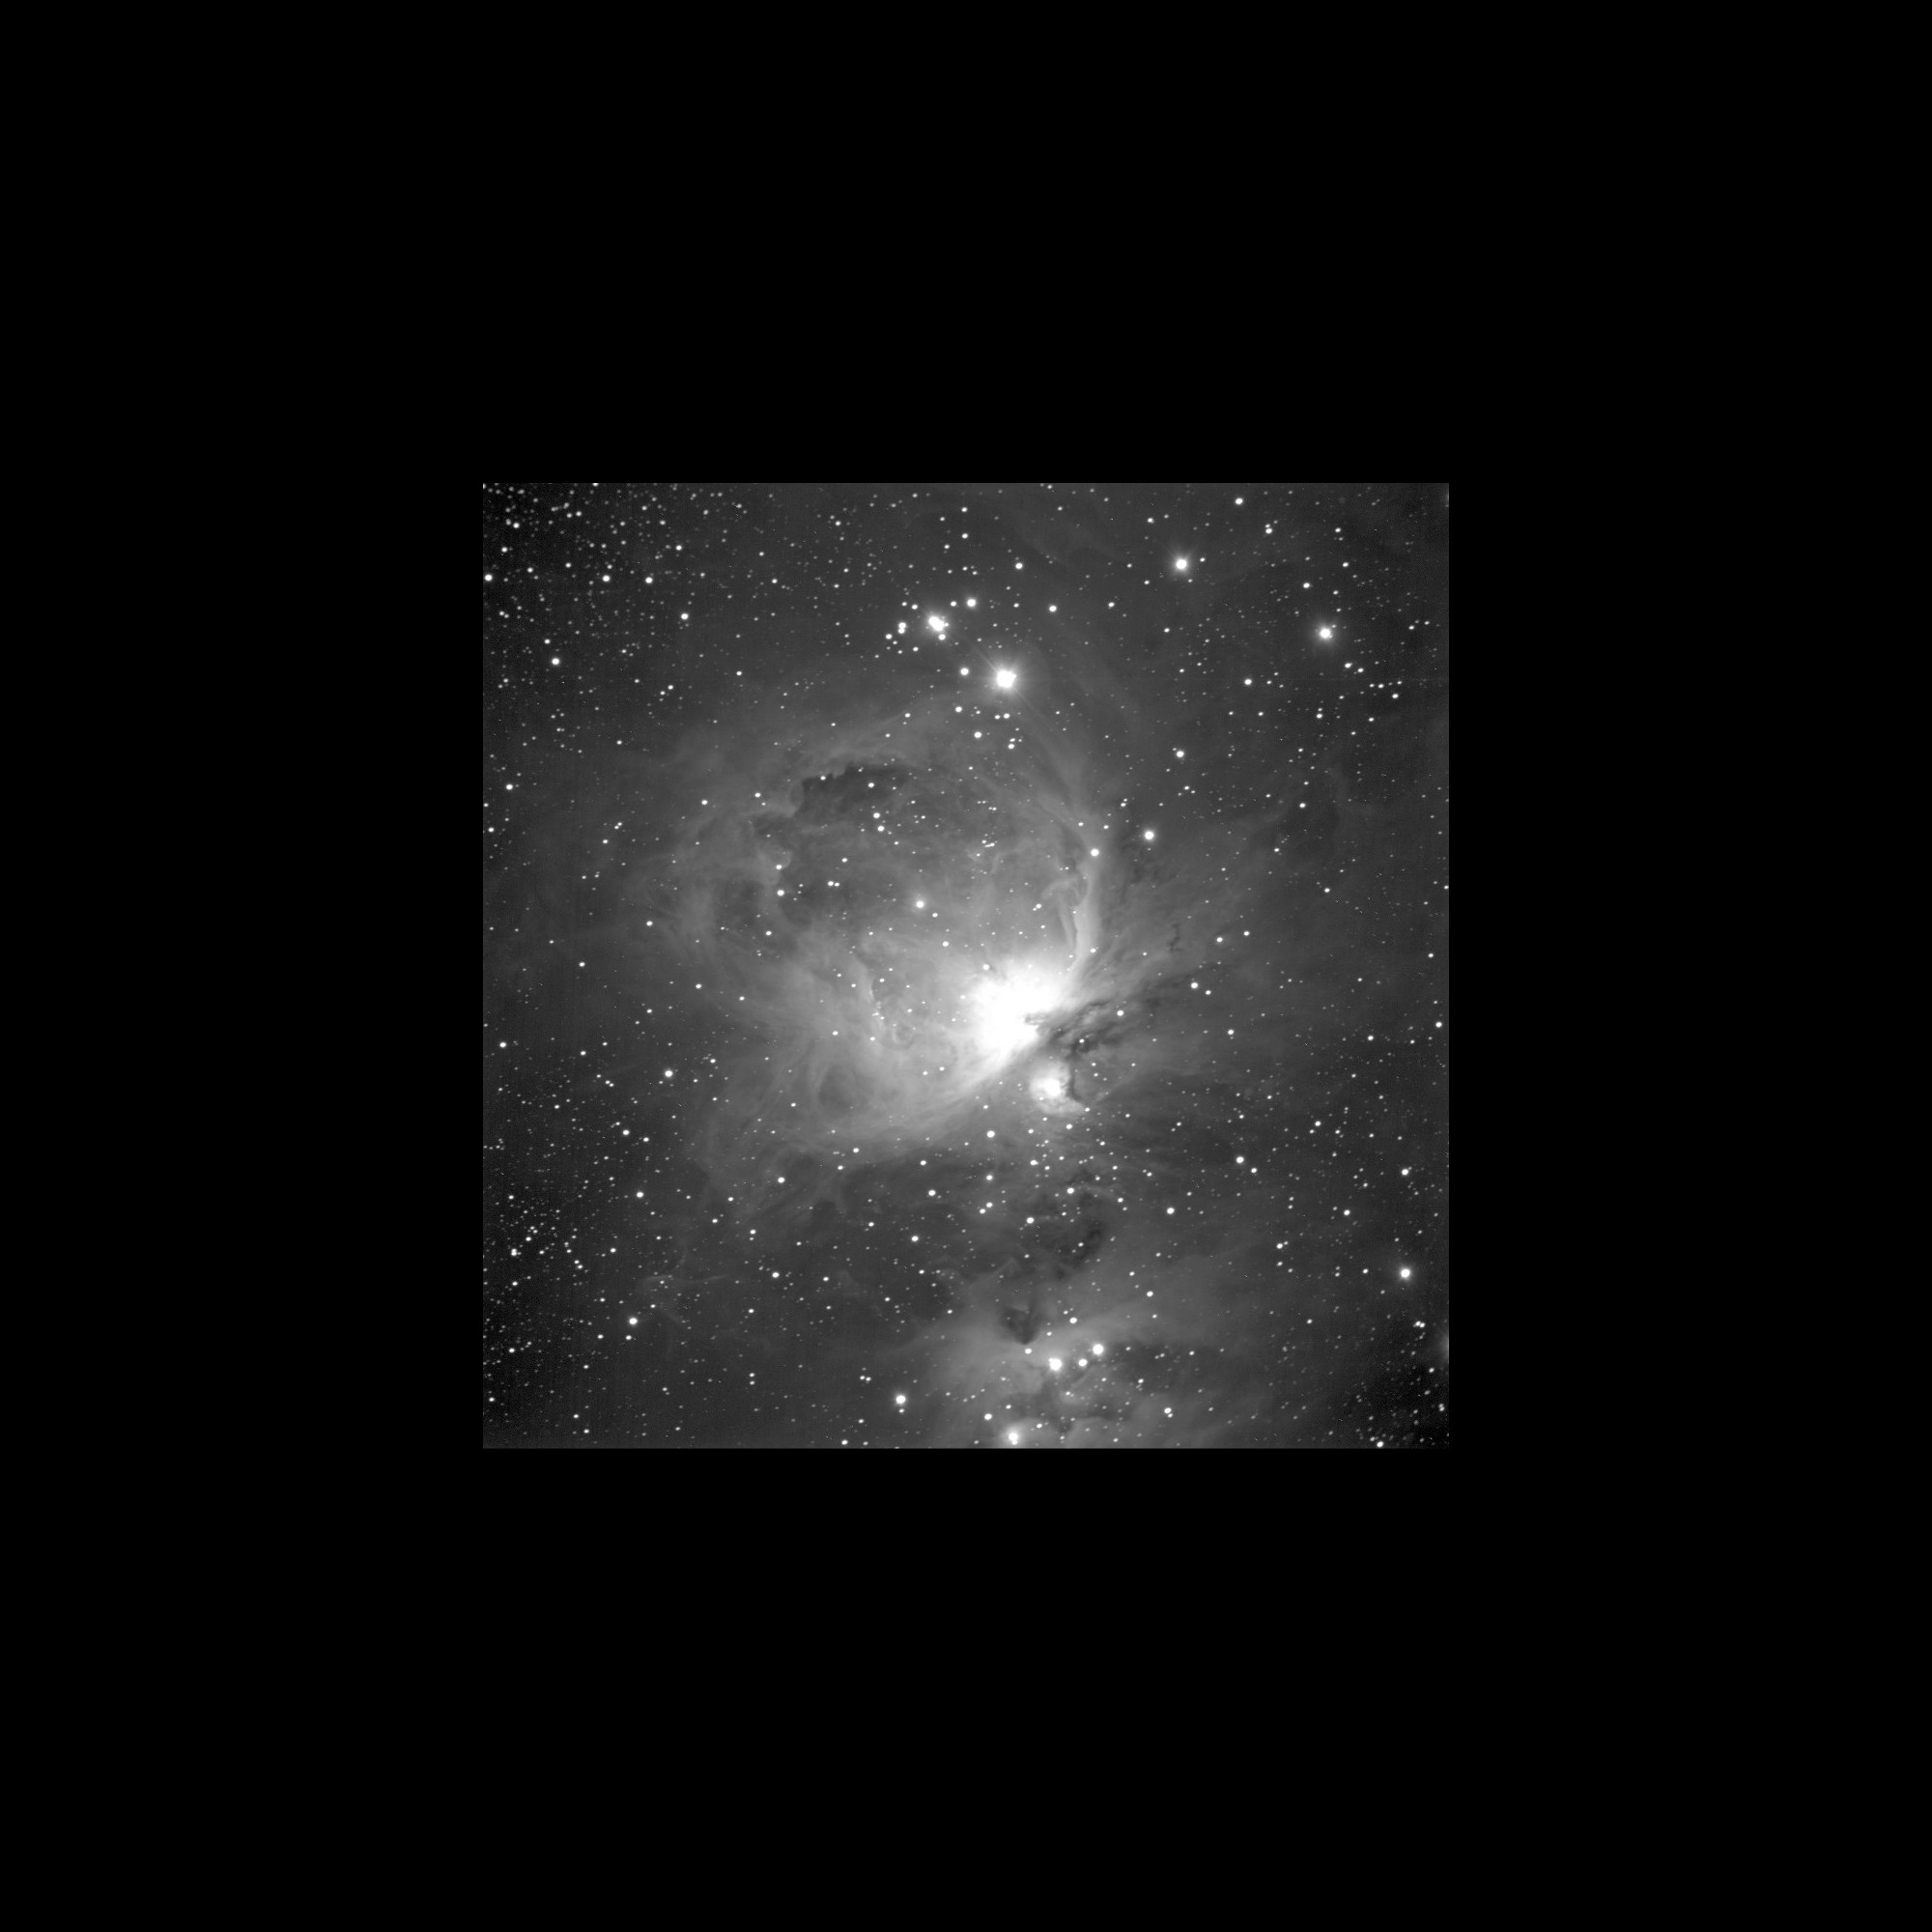
\includegraphics[width=6.6cm]{orion2.jpg}};
	\node[color=white] at (-3.3,3.3) [below right] {$u\mathstrut$};
	\begin{scope}
	\clip (-3.3,-3.3) rectangle (3.3,3.3);
	\foreach \a in {0,10,...,360}{
		\draw[color=red!10,shorten <= 0.1cm,line width=0.1pt]
			(\we:\re) -- +(\a:7);
	}
	\end{scope}
	\draw[color=red] (\w:\r) circle[radius=\d];
	\draw[color=blue] (\wb:\rb) circle[radius=\d];
	\draw[color=darkgreen] (\wc:\rc) circle[radius=\d];
	\draw[color=red!10] (\we:\re) circle[radius=\d];
\end{scope}

\begin{scope}[xshift=3.7cm,yshift=3.7cm]
	\node at (0,0) {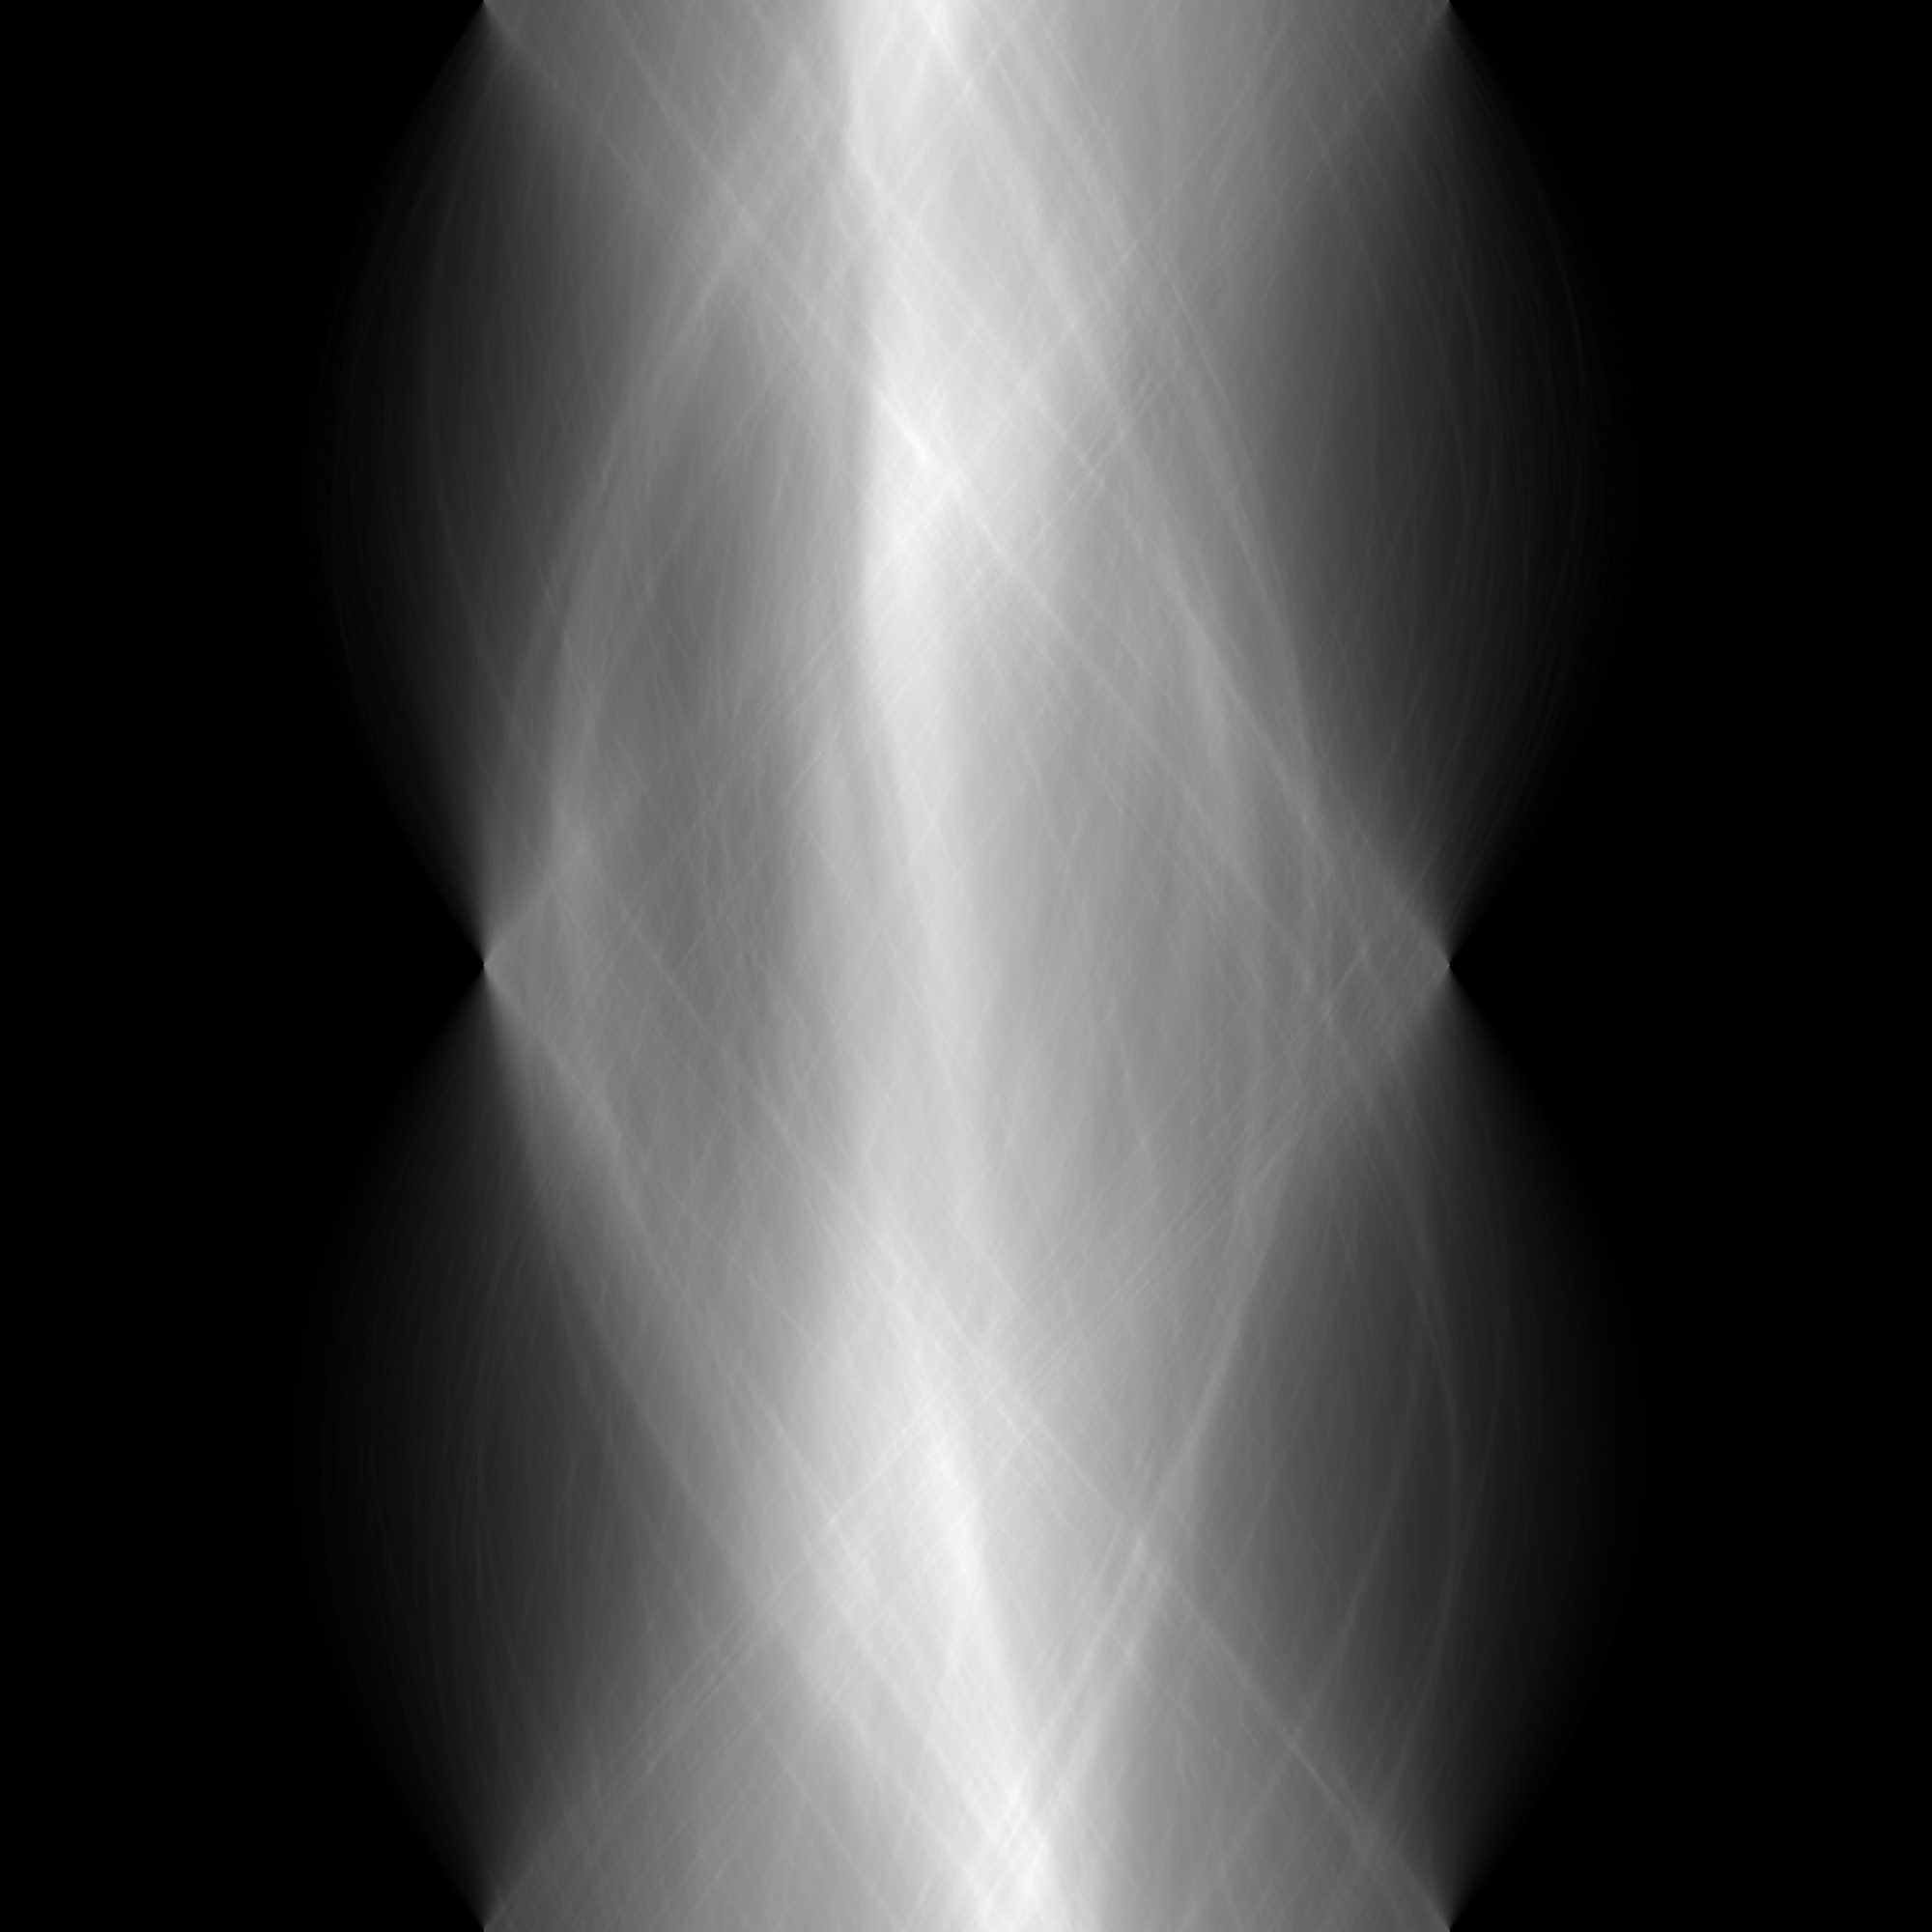
\includegraphics[width=6.6cm]{orion2-radon.jpg}};
	\node[color=white] at (3.3,3.3) [below left] {$\mathscr{R}u\mathstrut$};

	\draw[color=red,line width=0.2pt] plot[domain=0:180,samples=100] 
		({\r*cos(\x-\w)-\d},{-3.3+6.6*\x/180});
	\draw[color=red,line width=0.2pt] plot[domain=0:180,samples=100] 
		({\r*cos(\x-\w)+\d},{-3.3+6.6*\x/180});

	\draw[color=blue,line width=0.2pt] plot[domain=0:180,samples=100] 
		({\rb*cos(\x-\wb)-\d},{-3.3+6.6*\x/180});
	\draw[color=blue,line width=0.2pt] plot[domain=0:180,samples=100] 
		({\rb*cos(\x-\wb)+\d},{-3.3+6.6*\x/180});

	\draw[color=darkgreen,line width=0.2pt] plot[domain=0:180,samples=100] 
		({\rc*cos(\x-\wc)-\d},{-3.3+6.6*\x/180});
	\draw[color=darkgreen,line width=0.2pt] plot[domain=0:180,samples=100] 
		({\rc*cos(\x-\wc)+\d},{-3.3+6.6*\x/180});

\end{scope}


\begin{scope}[xshift=3.7cm,yshift=-3.7cm]
	\node at (0,0)
		{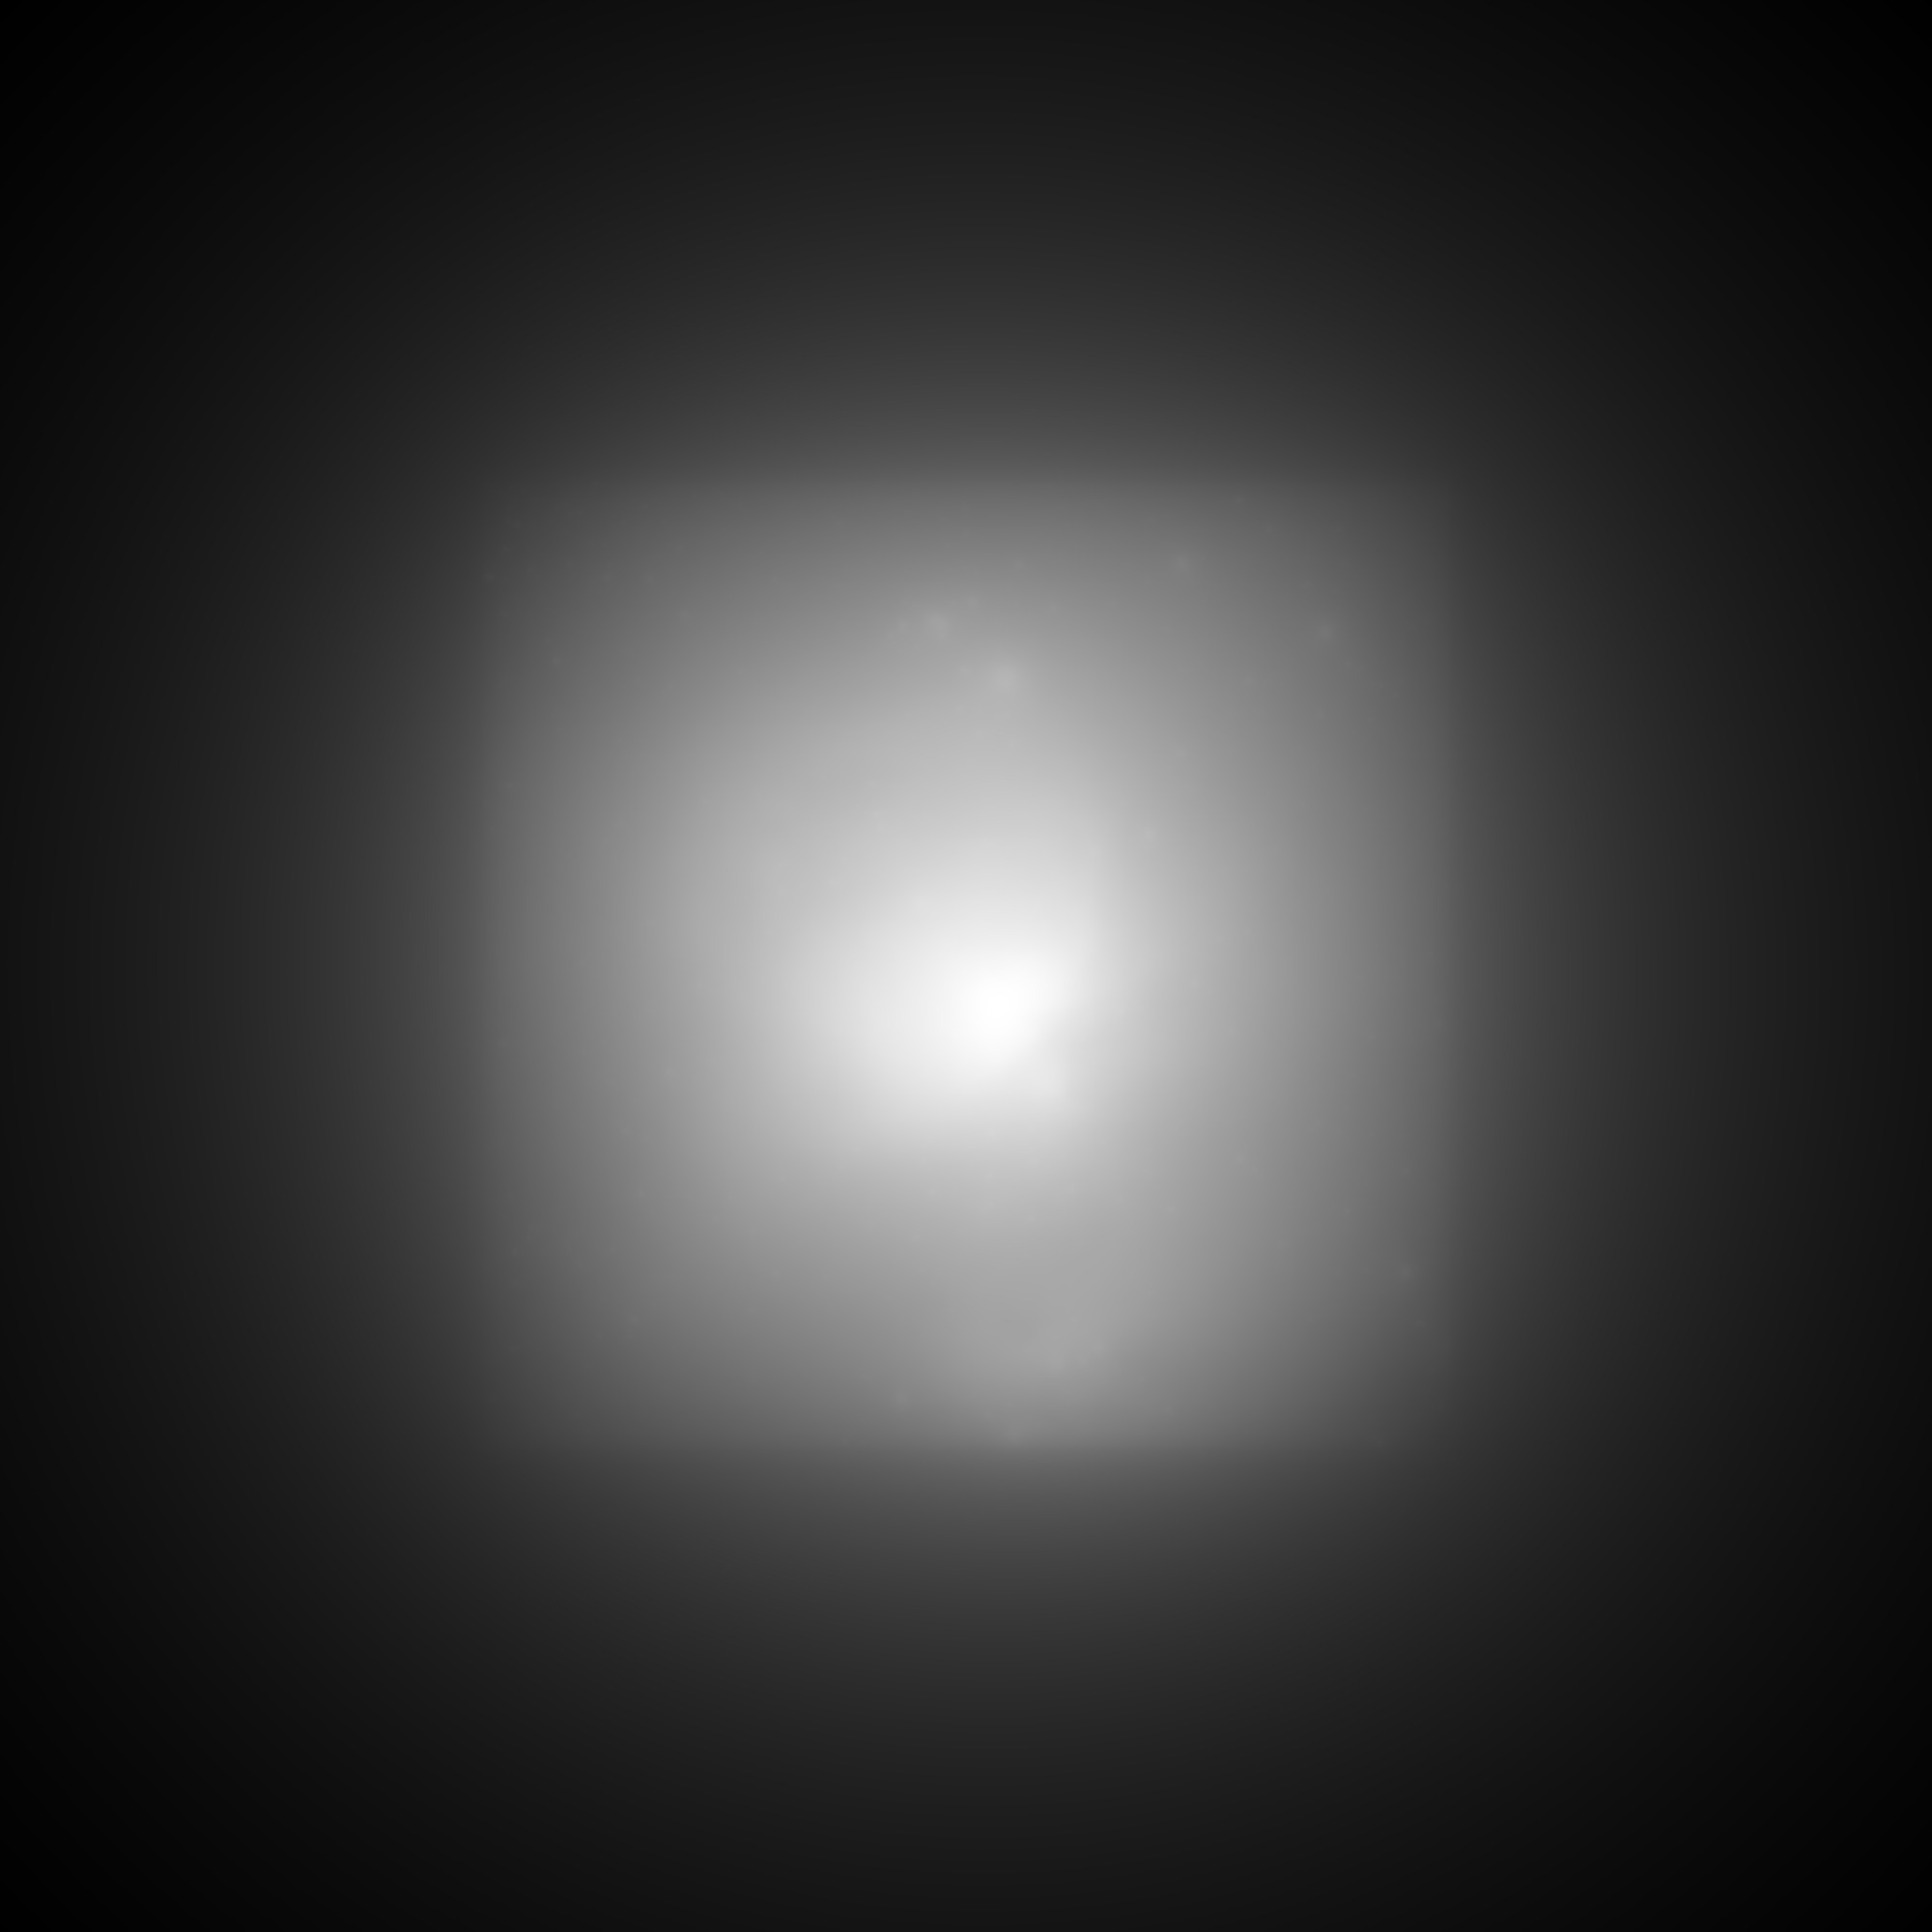
\includegraphics[width=6.6cm]{orion2-backprojection.jpg}};
	\node[color=white] at (3.3,-3.3) [above left]
		{$\mathscr{R}^*\mathscr{R}u\mathstrut$};
	\draw[color=red!10] (\we:\re) circle[radius={2*\d}];
\end{scope}

\begin{scope}[xshift=-3.7cm,yshift=-3.7cm]
	\node at (0,0) {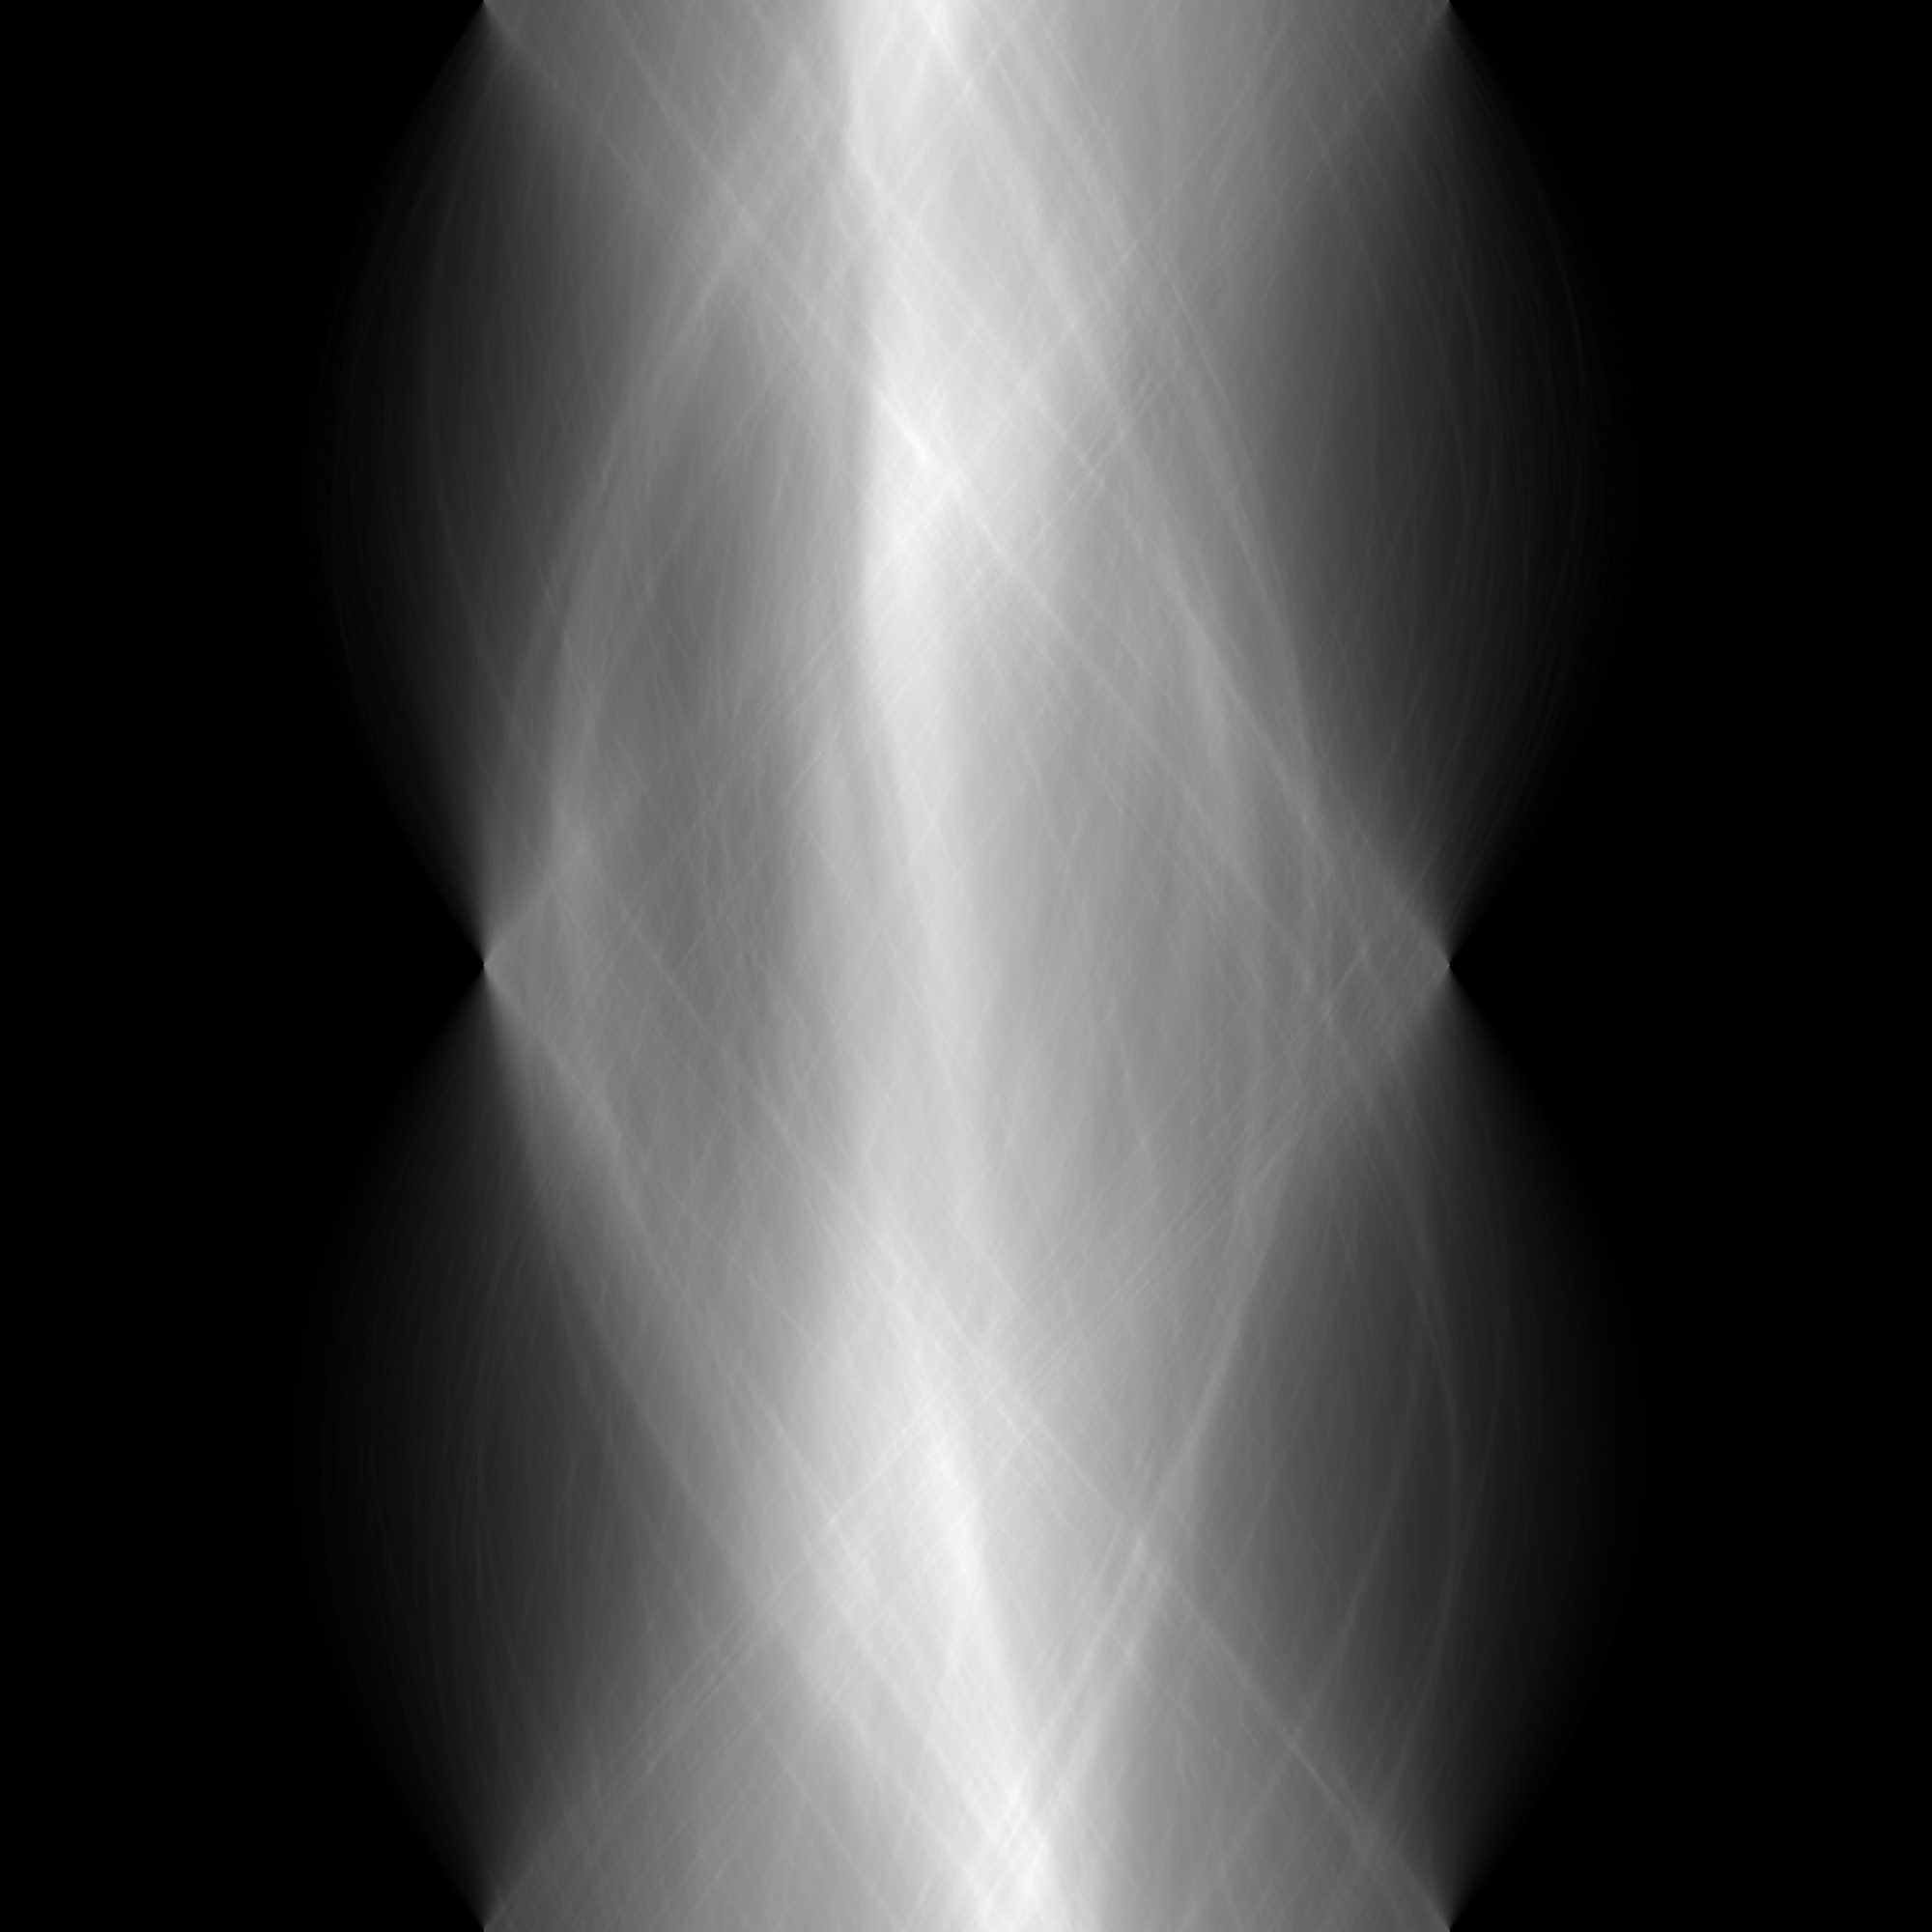
\includegraphics[width=6.6cm]{orion2-radon.jpg}};
	\node[color=white] at (-3.3,-3.3) [above right]
		{$\mathscr{R}u\mathstrut$};
	\begin{scope}
		\clip (-3.3,-3.3) rectangle (3.3,3.3);
		%\fill[color=red!10,opacity=0.1]
		%	plot[domain=0:180,samples=100] 
		%		({\r*cos(\x-\w)+\d},{-3.3+6.6*\x/180})
		%	--
		%	plot[domain=180:0,samples=100] 
		%		({\r*cos(\x-\w)-\d},{-3.3+6.6*\x/180})
		%	-- cycle;
		\foreach \a in {0,10,...,180}{
			\fill[color=red!10]
				({\re*cos(\a-\we)},{-3.3+6.6*\a/180})
					circle[radius=0.05];
		}
	\end{scope}
\end{scope}

\draw[->,color=white] (-1,3.7) -- (1,3.7);
\draw (-0.4,3.7) -- (0.4,3.7);
\node at (0,3.7) [above] {$\mathscr{R}$};

\draw[->,color=white] (-1,-3.7) -- (1,-3.7);
\draw (-0.4,-3.7) -- (0.4,-3.7);
\node at (0,-3.7) [below] {$\mathscr{R}^*$};

\draw[->,color=white] (-3.7,1) -- (-3.7,-1);
\draw[->] (-3.7,0.4) -- (-3.7,-1);
\node at (-3.7,0) [left] {$\mathscr{R}$};

\draw[->,color=white] (3.7,1) -- (3.7,-1);
\draw (3.7,1.0) -- (3.7,-0.4);
\node at (3.7,0) [right] {$\mathscr{R}^*$};

\end{tikzpicture}
\end{document}

